%!TEX root = ./main.tex

En esta seccion solo listaremos multiples resultados algebraicos que vienen desde el grupo de trenzas puro
\begin{theorem}
    Para $n\geq 2$, el grupo $U_n$ es libre generado por $A_{i,n}$, para $i=1,2,\ldots,n-1$
\end{theorem}
Este teorema es curiosamente de los mas utiles debido a que nos da una manera de reescribir elementos en $U_n$ y por consiguiente luego en $P_n$ de forma iterativa, esto se conoce como forma normal, este hecho nos da multiples corolarios supremamente interesantes, de los cuales enunciaremos dos
\begin{corollary}
    $P_n$ es libre de torsion, es decir no hay elementos de orden finito.
\end{corollary}
\begin{corollary}
    $P_n$ es generado por $A_{i,j}$ para $1\leq i<j\leq n$
\end{corollary}
Siguiendo esta idea en la seccion anterior explicitamente calculamos el centro de $B_3$ y vimos que era ciclico e infinito, resulta que de manera general tenemos que
\begin{theorem}
    Si $n\geq 3$ $Z(B_n)=Z(P_n)=\langle \Delta_n^2\rangle$, donde
    $$\Delta_n=(\sigma_1\sigma_2\cdots\sigma_{n-1})\cdots(\sigma_1\sigma_2)\sigma_1$$
\end{theorem}
Note que en particular para $n=3$, $\Delta_3=(\sigma_1\sigma_2)\sigma_1=x$, esta trenza de manera intuitiva se obtiene al fijar la parte superior y dar un giro de $\pi$ a los puntos inferiores
\begin{center}
    

\tikzset{every picture/.style={line width=0.75pt}} %set default line width to 0.75pt        

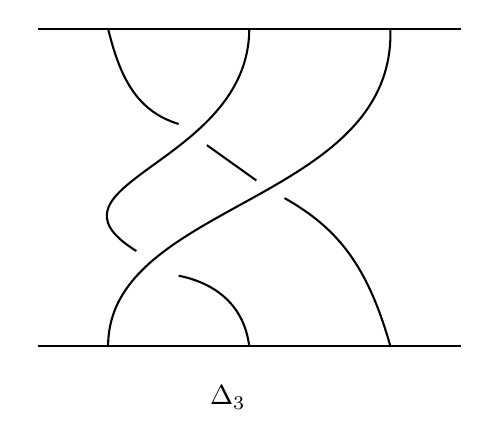
\begin{tikzpicture}[x=0.75pt,y=0.75pt,yscale=-1.7,xscale=1.7]
%uncomment if require: \path (0,877); %set diagram left start at 0, and has height of 877

%Curve Lines [id:da12746258618174844] 
\draw    (220,80) .. controls (221.5,129.5) and (140,129) .. (140,170) ;
%Curve Lines [id:da7267308029118377] 
\draw    (180,80) .. controls (180,118.5) and (117.5,124) .. (148,143) ;
%Curve Lines [id:da11813265743405121] 
\draw    (180,170) .. controls (178.5,158) and (170,152) .. (160,150) ;
%Curve Lines [id:da6401519497181539] 
\draw    (140,80) .. controls (143.5,94.5) and (148.5,103.5) .. (160,107) ;
%Curve Lines [id:da3785360469498672] 
\draw    (190,128) .. controls (205,136.5) and (213.5,147) .. (220,170) ;
%Straight Lines [id:da5224494229876718] 
\draw    (168,113) -- (182,123) ;
%Straight Lines [id:da422154150629262] 
\draw    (120,80) -- (240,80) ;
%Straight Lines [id:da5681564586047843] 
\draw    (120,170) -- (240,170) ;

% Text Node
\draw (168,180.4) node [anchor=north west][inner sep=0.75pt]    {$\Delta _{3}$};


\end{tikzpicture}
\end{center}
 De este hecho se sigue un corolario que aunque intuitivamente tenia mucho sentido no lo habiamos probado aun
 \begin{corollary}
     Para $m\neq n$, $B_m$ no es isomorfo a $B_n.$
 \end{corollary}

 Por ultimo no es un corolario directo de esto ya que depende del espacio de configuración pero también es un hecho estándar.
 \begin{theorem}
     $B_n$ es un grupo libre de torsión.
 \end{theorem}
 \subsection{El espacio $C_n(\R^2)$}
 Finalizamos con una breve descripción del espacio de configuración por medio de polinomios, que nos da una relación muy interesante hacia la geometría algebraica. Si hacemos la identificación natural de $\R^2=\C$, consideremos el siguiente polinomio simétrico
 $$p_k(u)=(-1)^k\sum_{1\leq i_1<\cdots<i_k\leq n}u_{i_1}\cdots u_{i_k}.$$
 Donde $u\in \mathcal{F}_n(\C)$ y $k=1,\ldots n$, note que por ser simétrico estas funciones $p_k$ son invariantes bajo la acción de $S_n$, por lo que inducen una función $C_n(\C)\to \C^n $. Resulta que esta función es un homeomorfismo al conjunto de los polinomios monoicos con raíces diferentes de grano $n$ y coeficientes complejos. Siendo así $B_n$ el grupo fundamental de un conjunto clásico en la geometría algebraica.
